\chapter{Surface Data}
\label{ch:App:surface data}

\begin{table}[h]
\centering
\caption{Surface data}
\label{tab:surface data}
\begin{tabular}{|l|c|}
\hline
                        & \begin{tabular}[c]{@{}c@{}}Surface Fluxes\\  W/m2\end{tabular} \\ \hline
Floor-South             & -172.0                                                         \\ \hline
Floor-North             & -158.1                                                         \\ \hline
South Wall              & -25.7                                                          \\ \hline
East Wall               & -29.3                                                          \\ \hline
West Wall-South         & -33.1                                                          \\ \hline
West Wall-North         & -130.6                                                         \\ \hline
North Wall-Bottom       & -58.0                                                          \\ \hline
North Wall-Below Window & -166.7                                                         \\ \hline
Window                  & -201.7                                                         \\ \hline
North Wall-Above Window & 52.3                                                           \\ \hline
Ceiling                 & 227.6                                                          \\ \hline
Sauna-South Face        & 166.4                                                          \\ \hline
Sauna-East Face         & 187.7                                                          \\ \hline
Hot Rocks               & 5343.1                                                         \\ \hline
\end{tabular}
\end{table}

\chapter{Other important information}
\lipsum[3]

\begin{figure}[htbp!]
    \centering
    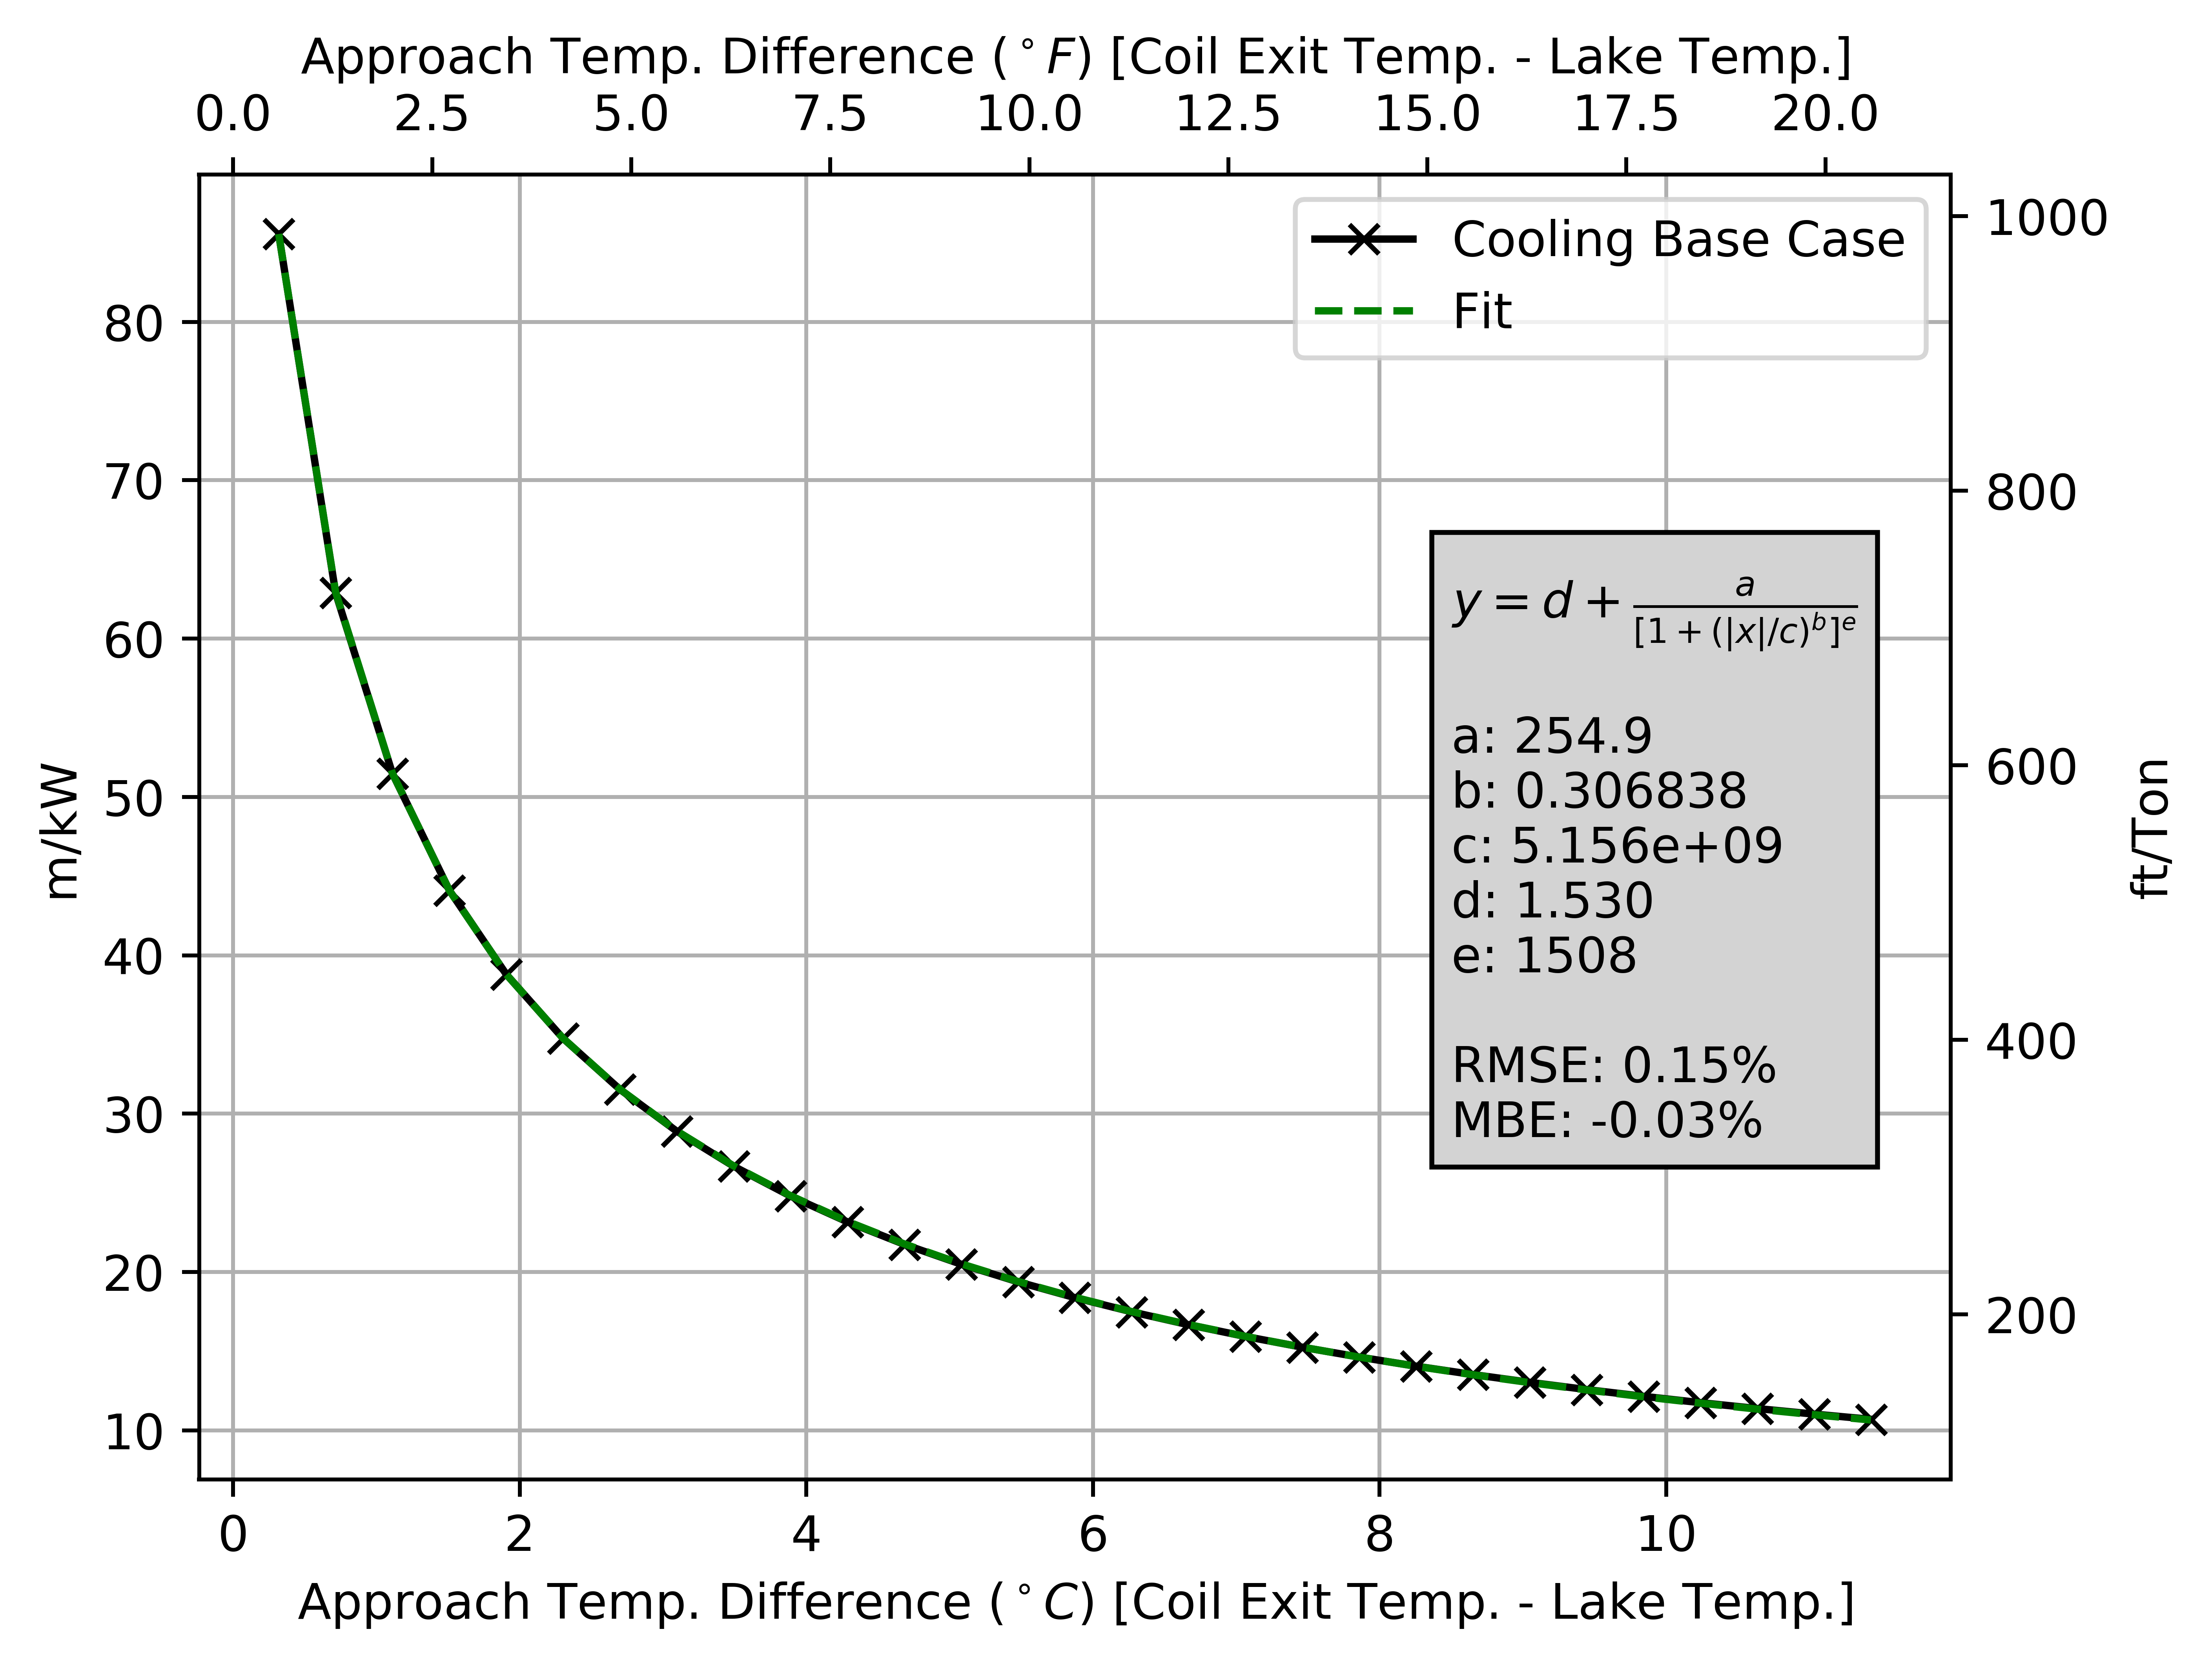
\includegraphics[width=0.75\textwidth]{Cooling_BaseCase_CurveFit.png}
    \caption{Another cool figure (in the appendix)}
    \label{fig:another cool figure in appendix}
\end{figure}
